\section{Vistas}

Pasaremos a ahora a presentar los distintos diagramas para continuar modelizando nuestro problema.

En una primera instancia presentaremos el diagrama de clases, si bien presentamos el diagrama no estará acompañado de sus predicados de OCL, estos se presentaran posteriormente en la vista de las distintas etapas. 
Como dijimos anteriormente, presentaremos nuestra solución dividiendola en 3 etapas: Preparación, sufragio y conteo. 

Contamos con 5 tipos de diagramas, analizemos un poco las ventajas y desventajas de cada uno antes de comenzar.

\paragraph{Diagrama de contexto} 

El diagrama de contexto es una de las piedras angulares de este trabajo, nos permite observar las interacciones entre agentes. A su vez, no tenemos orden de las acciones ni una relación temporal lo cual nos impide modelizar muchas situaciones.

\paragraph{Diagrama de clases y OCL}

El diagrama de clases nos presenta una visión general de lo que vamos a modelizar, a su vez nos define un poco más las relaciones entre las clases de nuestro sistema. Permite dar una panorama general de como se comportan las clase entre ellas y que se le atribuye a cada una. Al mismo tiempo, el diagrama no permite expresar todo, para esto usaremos OCL, un lenguaje que expande al diagrama y nos permite expresar más relaciones entre clases.

\paragraph{Diagrama de casos de uso}

Este diagrama nos permite describir la interacción entre el sistema y los distintos actores 
externos. Junto a la descripción de los casos de uso, construye un detalle importante para la 
construcción del sistema.

\paragraph{Diagrama de Actividad}

El diagrama de actividad pone un orden relativo en los casos de uso. Y los relaciona aún más con los actores.

\paragraph{Máquinas de estado finitas}

La máquina de estados permite la composición entre varios actores con el mismo comportamiento y a su vez nos permite dar un orden temporal de los eventos. 


Presentaremos primero el diagra de contexto y el diagrama de clases.

\subsection{Diagrama de Contexto}
\todo[inline]{Aca va el diagrama de contexto}


\subsection{Diagrama de Clases}
\todo[inline]{Aca va el diagrama de clases}

Ya presentados el diagrama de contexto y el de clases podemos pasar a analizar para cada una de las etapas presentadas en la introducción mediante los distintos diagramas ya presentados.

\subsection{Preparación}


\subsubsection{Diagrama de actividad}

\todo[inline]{PONER EN SU LUGAR LOS DIAGRAMAS DE ACTIVIDAD}
\begin{figure}[h!]
\centering
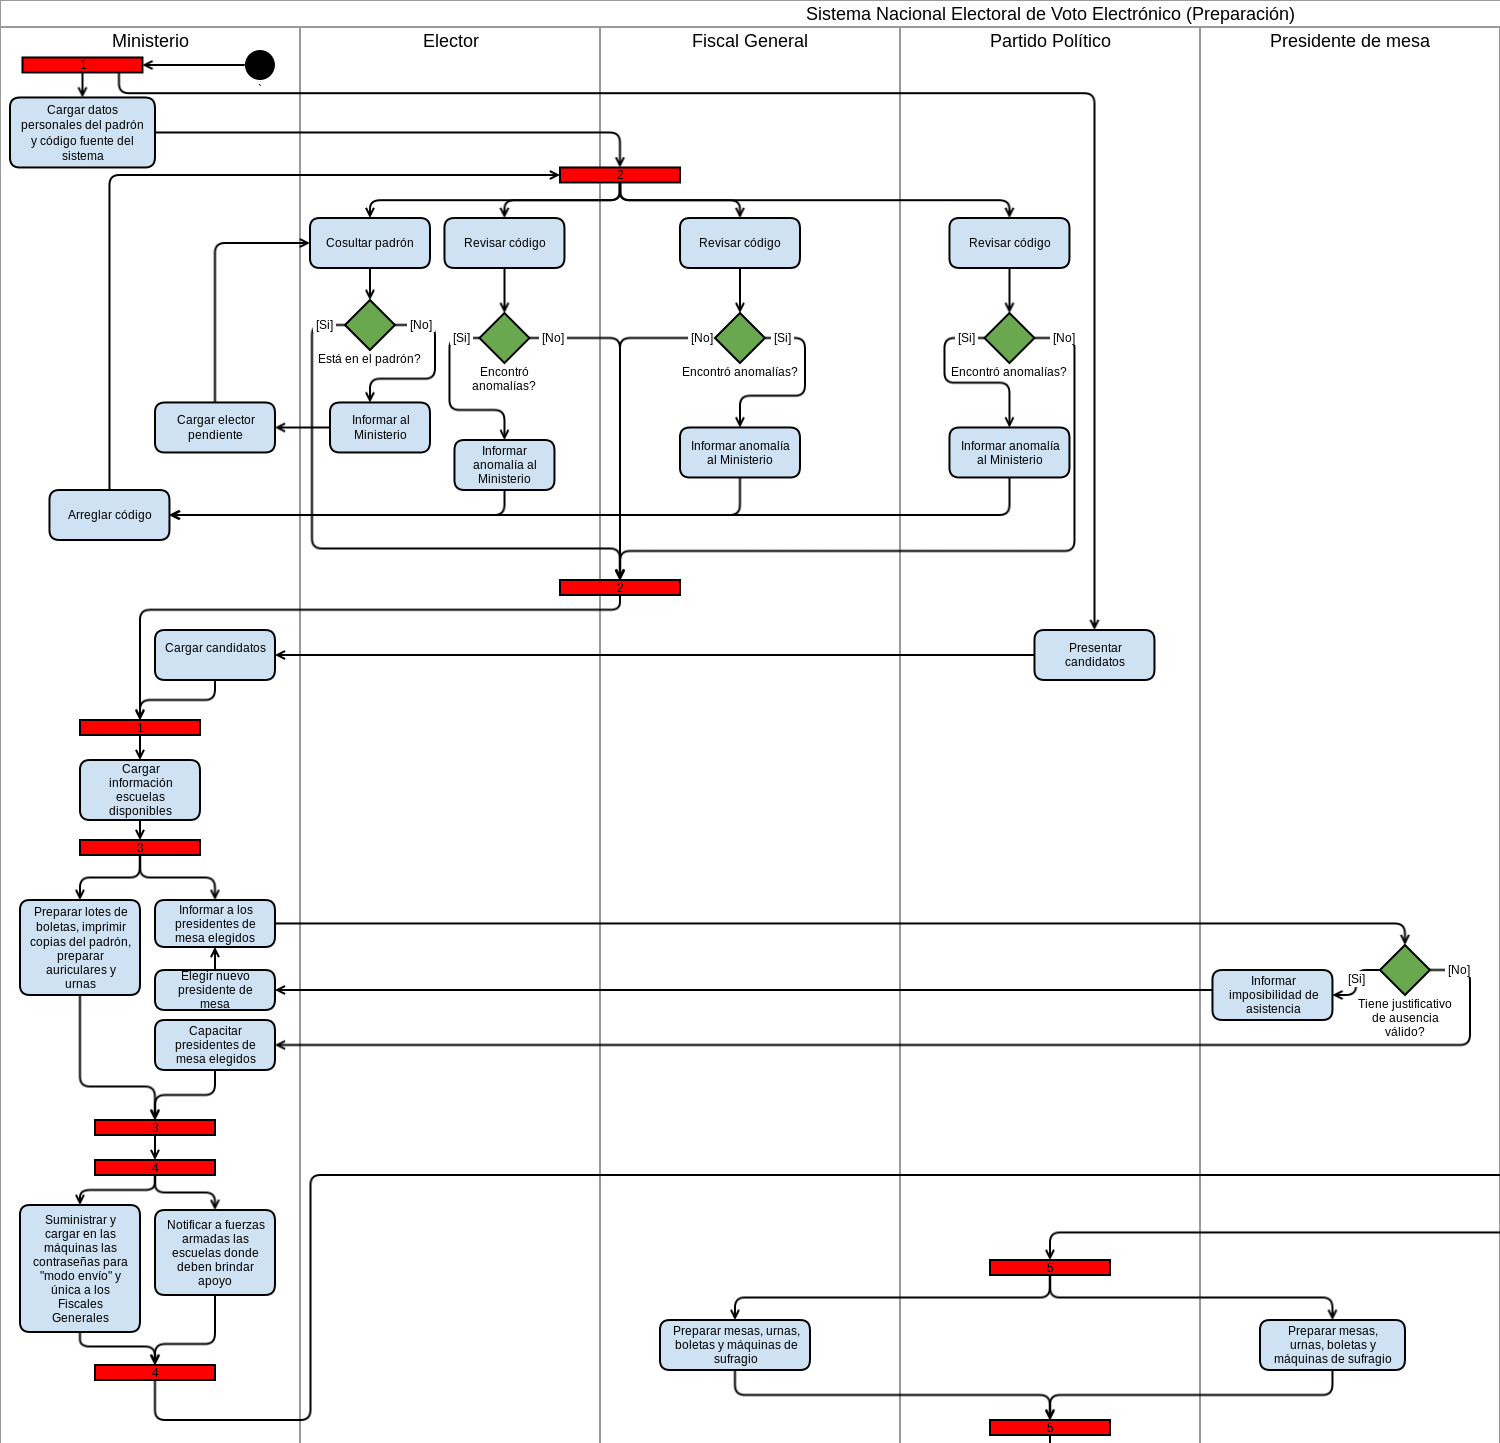
\includegraphics[scale=0.5]{imagenes/actividad/actividadPreparacion1}
%\captionof{figure}{Diagrama de actividad}
\end{figure}

\begin{figure}[h!]
\centering
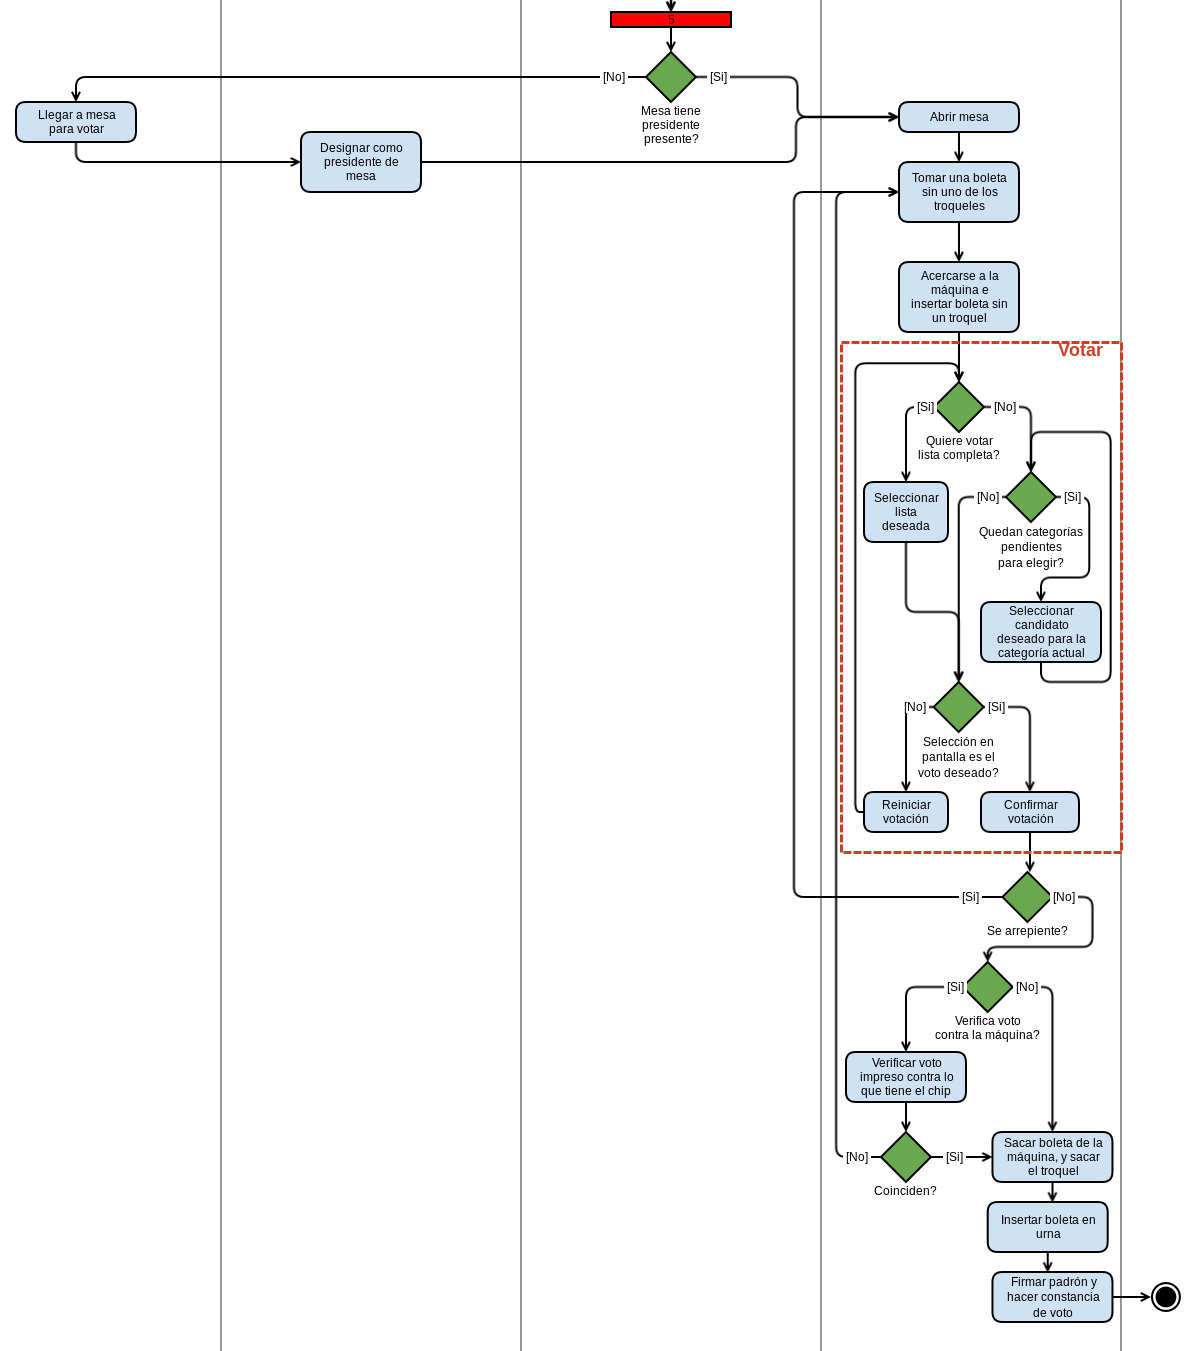
\includegraphics[scale=0.5]{imagenes/actividad/actividadPreparacion2}
\end{figure}

\begin{figure}[h!]
\centering
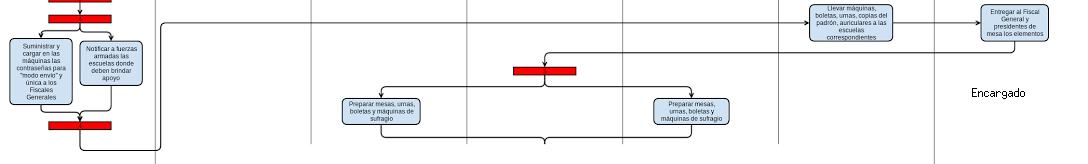
\includegraphics[scale=0.5]{imagenes/actividad/actividadPreparacion3}
\end{figure}

\subsubsection{Máquina de estado finito}

Para esta sección fu necesario construir 2 máquinas de estado.

\begin{figure}[H]
\centering
%\includegraphics[scale=0.45]{}
%\captionof{figure}{Máquina de fechas limite}
\end{figure}

Esta máquina de estado nos define los tiempos de la etapa, es decir enmarca los tiempos de los casos de uso presentados anteriormente.

\begin{figure}[H]
\centering
%\includegraphics[scale=0.45]{}
%\captionof{figure}{Máquina de elección aleatoria de presidente de mesa}
\end{figure}


\subsubsection{Casos de uso}

\textbf{Caso de Uso: Autenticandose}

\textbf{Actores:} Ministerio

\textbf{Pre:} -

\textbf{Post:} El ministerio se encuentra autenticado en el sistema web.
\begin{table}[h!]
	
 \begin{tabular}{|p{7.5cm} | p{7.5cm}|} 
 \hline
 \textbf{Curso normal} & \textbf{Curso Alternativo} \\
 \hline
 %\hline
 1. El ministerio ingresa al sistema web. & \\
 \hline
 
 2. El sistema le pide usuario y contraseña para ingresar. & \\
 \hline 
 3. El ministerio ingresa usuario y contraseña, y elige la opción “Ingresar”. & \\
 \hline 
 4. La información se valida, y se muestra el menú principal. & 
4.1. La información de inicio no es correcta, por lo que se muestra un mensaje de error. Ir al paso 2.
\\
 \hline 
 5. Fin de CU. & \\

 \hline
 \end{tabular}

\end{table}


\textbf{Caso de Uso: Ingresando nuevo votante}

\textbf{Actores:} Ministerio

\textbf{Pre:} El ministerio se encuentra autenticado en el sistema, el padrón se encuentra cargado en el sistema, y puede ser consultado desde la web.

\textbf{Post:} El padrón se actualiza en el sistema, agregando al nuevo votante.
\begin{table}[h!]
	
 \begin{tabular}{|p{7.5cm} | p{7.5cm}|} 
 \hline
 \textbf{Curso normal} & \textbf{Curso Alternativo} \\
 \hline

1. El ministerio ingresa los datos del nuevo votante en un formulario. & \\
\hline

2. El ministerio elige la opción de “Cargar votantes”. & \\
\hline

3. Se actualizan los datos en el sistema. & 3.1. Si existe un error en la carga, se muestra un mensaje con el error. Ir al paso 2. \\
\hline
4. Fin de CU. & \\
 \hline
 \end{tabular}

\end{table}


\textbf{Caso de Uso: Consultando presidentes de mesa}

\textbf{Actores:} Ministerio 

\textbf{Pre:} El ministerio se encuentra autenticado en el sistema, las mesas y los presidentes de mesa se encuentra publicados.

\textbf{Post:} El ministerio conoce a los presidentes de mesa.
\begin{table}[h!]
	
 \begin{tabular}{|p{7.5cm} | p{7.5cm}|} 
 \hline
 \textbf{Curso normal} & \textbf{Curso Alternativo} \\
 \hline

1. El ministerio selecciona la pestaña de consulta de presidentes de mesa. & \\
\hline
2. El ministerio consulta en el sistema los presidentes asignados a cada mesa. & \\
\hline
3. Fin de CU. & \\
\hline
 \end{tabular}

\end{table}

\textbf{Caso de Uso: Asignando nuevo presidente de mesa}

\textbf{Actores:} Ministerio 

\textbf{Pre:} El ministerio se encuentra autenticado en el sistema, las mesas y los presidentes de mesa se encuentran publicados, y un presidente de mesa envió una notificación explicando que no puede estar presente. La notificación se envió llamando a la línea gratuita del ministerio.

\textbf{Post:} Se asigna un nuevo presidente a una mesa.
\begin{table}[h!]
	
 \begin{tabular}{|p{7.5cm} | p{7.5cm}|} 
 \hline
 \textbf{Curso normal} & \textbf{Curso Alternativo} \\
 \hline

1. El ministerio activa la opción de una nueva asignación de presidente de mesa para la mesa afectada. & \\
\hline

2.  El sistema aleatoriamente elige un presidente de mesa, descartando al presidente ya elegido, y priorizando a aquellos que no lo fueron previamente. & \\
\hline


3. Fin de CU. & \\
\hline



 \end{tabular}

\end{table}


\textbf{Caso de Uso: Consultando notificaciones de error en código fuente}

\textbf{Actores:} Ministerio 

\textbf{Pre:} El ministerio se encuentra autenticado en el sistema y el código fuente se encuentra publicado.
\textbf{Post:} El ministerio conoce las notificaciones de error sobre el código fuente.


\begin{table}[h!]
	
 \begin{tabular}{|p{7.5cm} | p{7.5cm}|} 
 \hline
 \textbf{Curso normal} & \textbf{Curso Alternativo} \\
 \hline


1. El ministerio selecciona la pestaña de notificaciones. & \\
\hline


2. El ministerio ministerio revisa todas las notificaciones cargadas en el sistema. & \\
\hline


3. Si se decide corregir uno de los errores cargados, se extiende con el CU \textbf{Corrigiendo código fuente}. & \\
\hline


4. Fin de CU. & \\
\hline




 \end{tabular}

\end{table}



\textbf{Caso de Uso: Iniciando votación}

\textbf{Actores:} Presidente de mesa

\textbf{Pre:} Es el día de la votación y ya se encuentra todo preparado en la mesa.

\textbf{Post:} La máquina ya se puede utilizar para votar, y el presidente de mesa ya votó.

\begin{table}[h!]
	
 \begin{tabular}{|p{7.5cm} | p{7.5cm}|} 
 \hline
 \textbf{Curso normal} & \textbf{Curso Alternativo} \\
 \hline

1. El presidente de mesa conecta la máquina de sufragio a la red eléctrica. & \\
\hline
2. El presidente de mesa prende la máquina de sufragio y activa el modo votación. & \\
\hline
3. El presidente de mesa vota de acuerdo a lo explicado en el CU Votando del Elector. & \\
\hline
4. Fin de CU.& \\
\hline



 \end{tabular}

\end{table}

\subsubsection{OCL}





\subsection{Sufragio}

\subsubsection{Máquina de estado finito}

\subsubsection{Diagrama de actividad}
\todo[inline]{PONER EN SU LUGAR LOS DIAGRAMAS DE ACTIVIDAD}
\begin{figure}[h!]
\centering
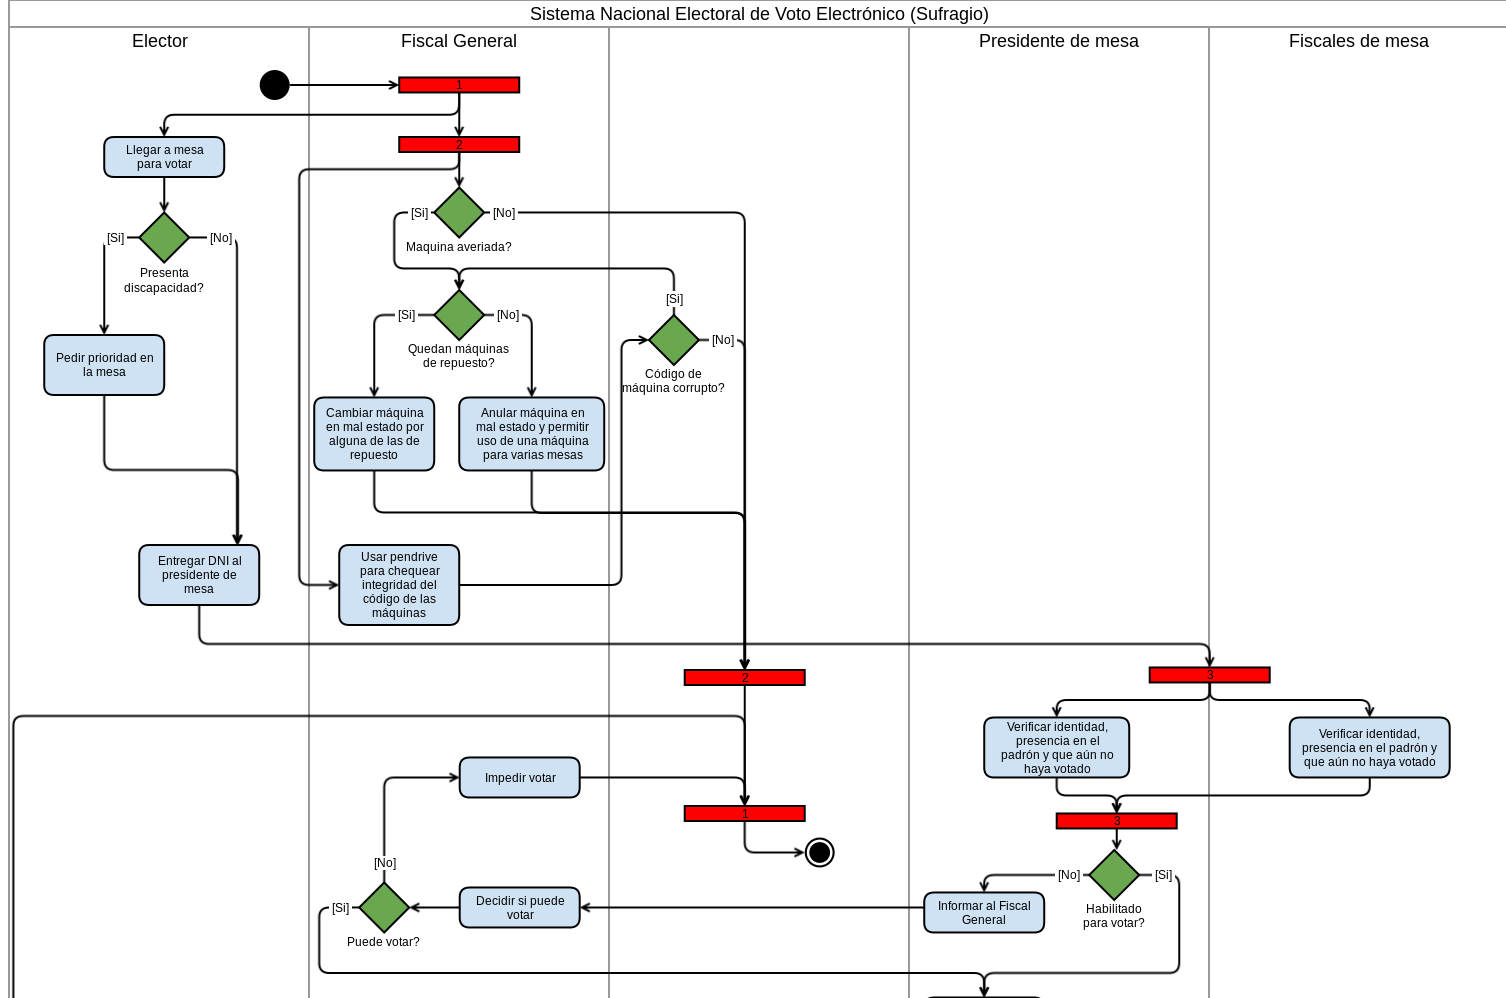
\includegraphics[scale=0.5]{imagenes/actividad/actividadSufragio1}
%\captionof{figure}{Diagrama de actividad}
\end{figure}

\begin{figure}[h!]
\centering
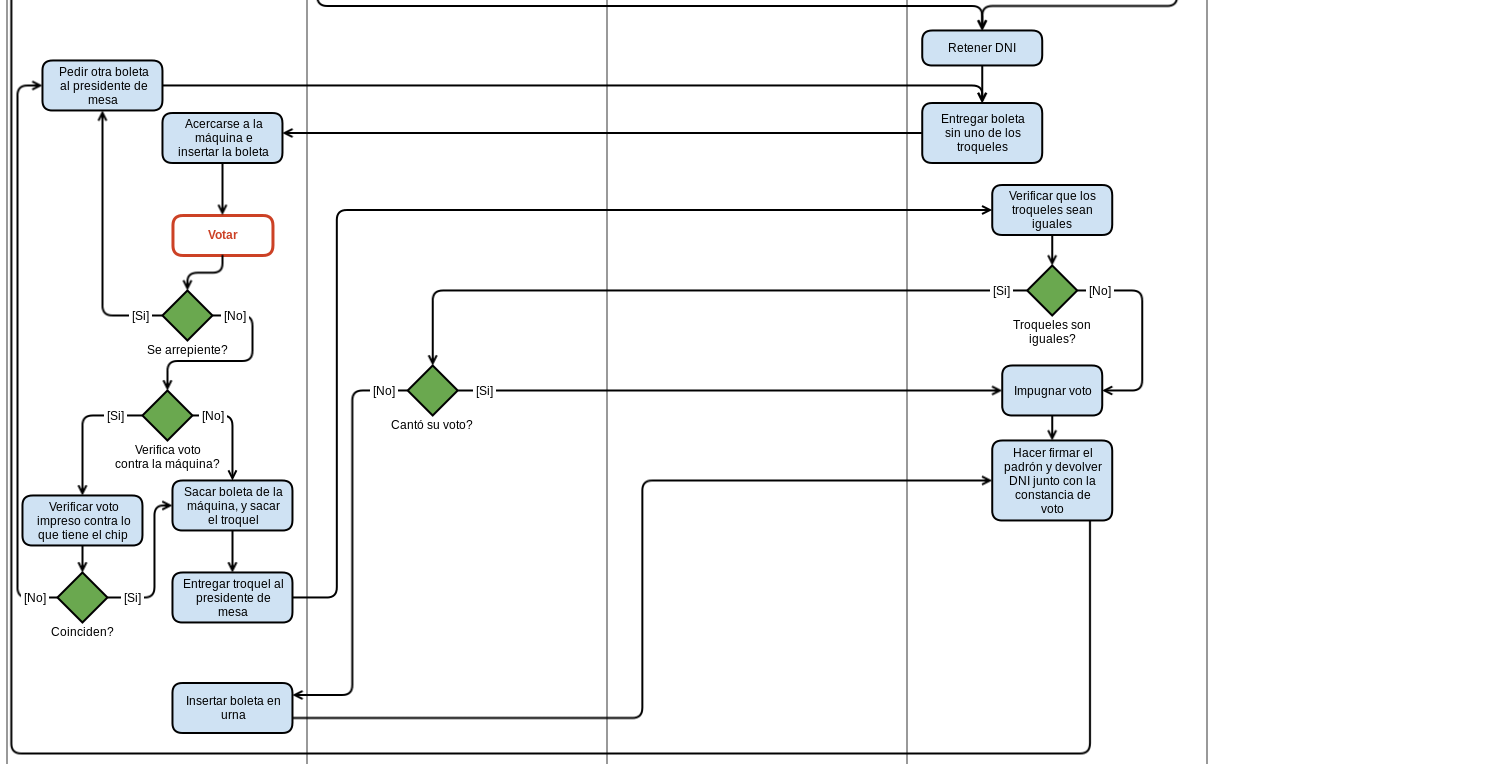
\includegraphics[scale=0.5]{imagenes/actividad/actividadSufragio2}
\end{figure}

\subsubsection{Casos de uso}

\subsubsection{OCL}

\subsection{Conteo}

\subsubsection{Máquina de estado finito}

\subsubsection{Diagrama de actividad}
\todo[inline]{PONER EN SU LUGAR LOS DIAGRAMAS DE ACTIVIDAD}
\begin{figure}[h!]
\centering
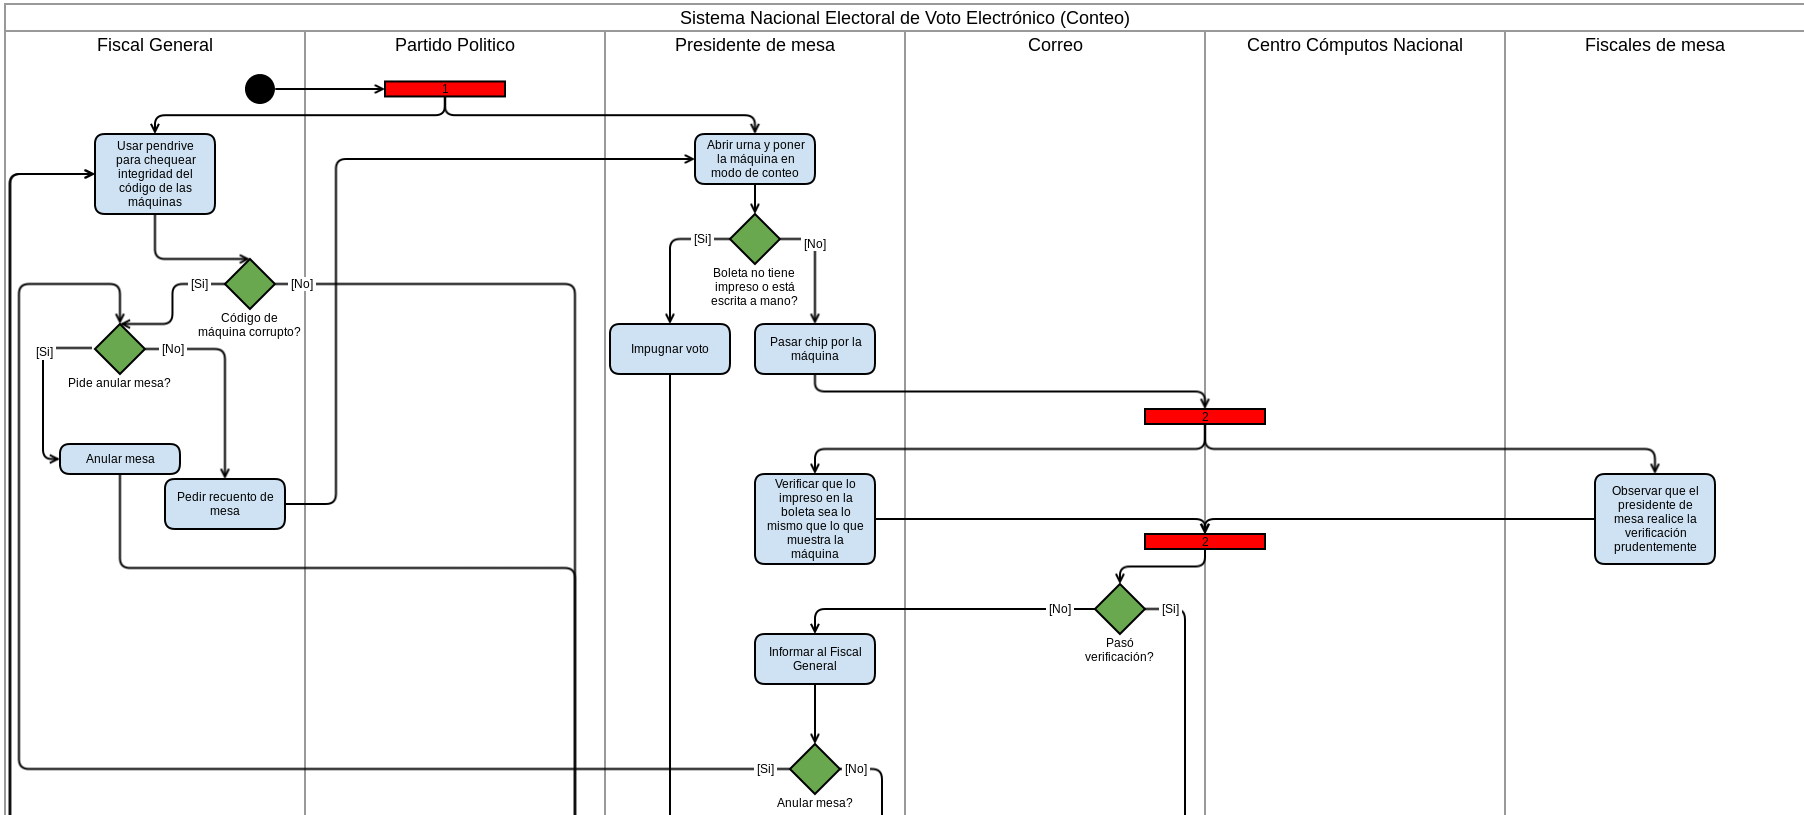
\includegraphics[scale=0.5]{imagenes/actividad/actividadConteo1}
%\captionof{figure}{Diagrama de actividad}
\end{figure}

\begin{figure}[h!]
\centering
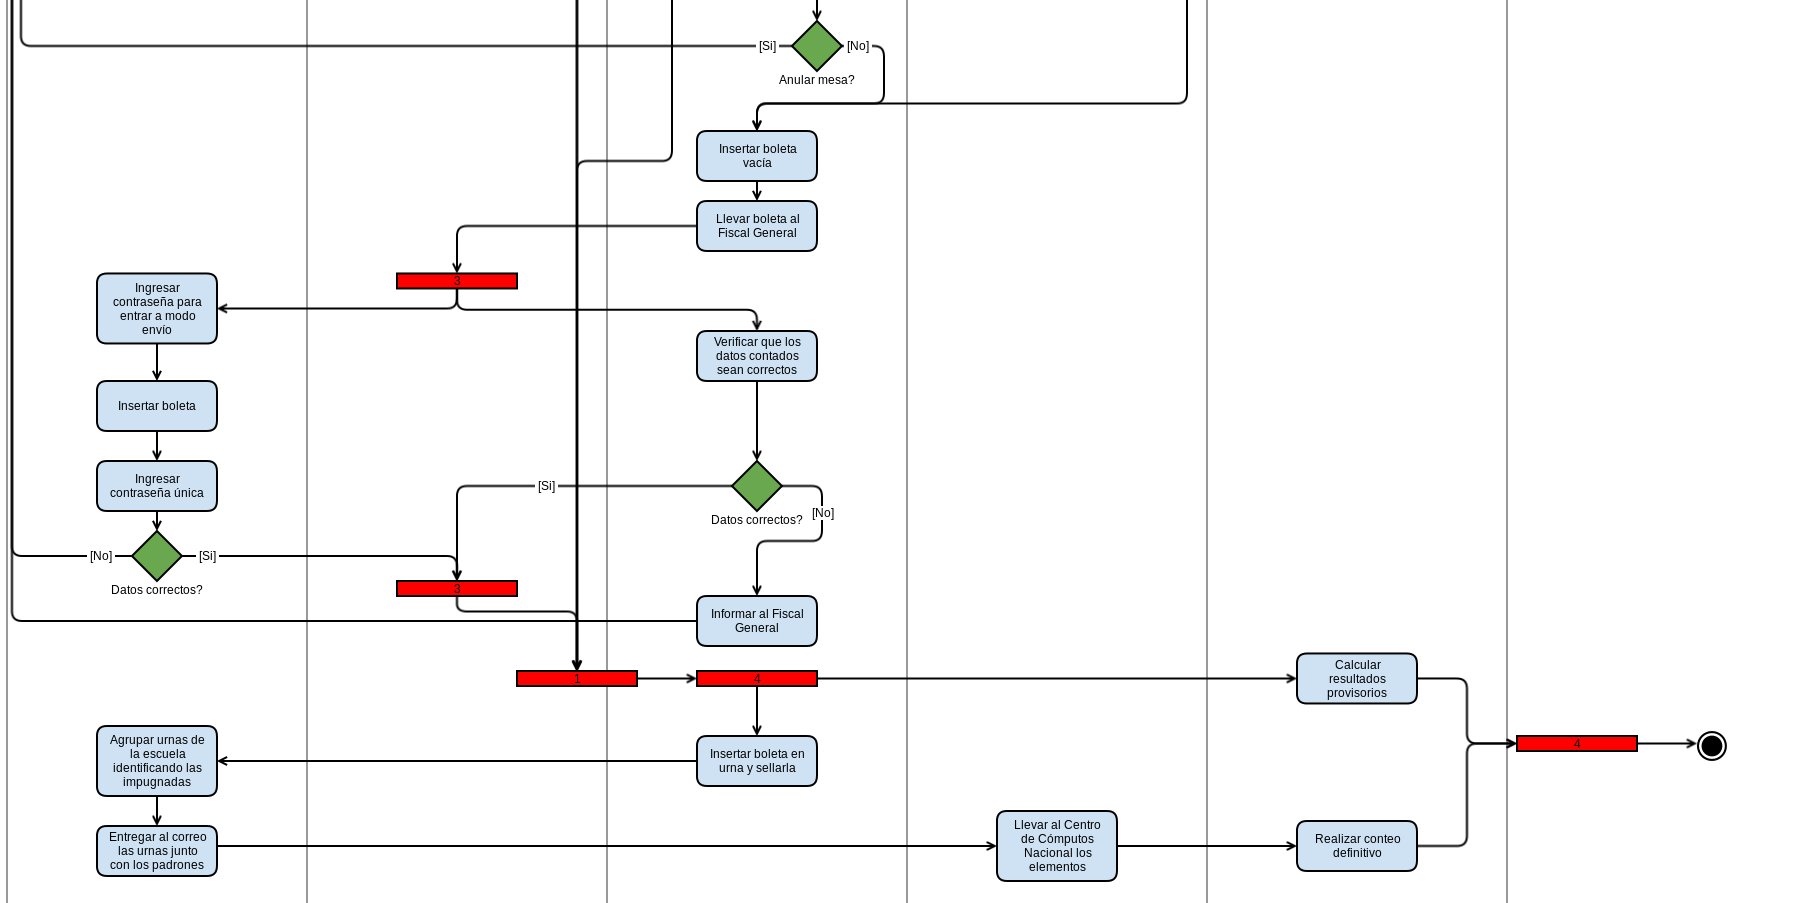
\includegraphics[scale=0.5]{imagenes/actividad/actividadConteo2}
\end{figure}


\subsubsection{Casos de uso}


\subsubsection{OCL}